% =========================================================================
\section{Design Models and Diagrams}
\label{sec:models}
% =========================================================================

\subsection{Data Flow Diagrams}
\subsubsection{Level 0 (context)}
Figure~\ref{fig:dfd0} shows \mahros{} as a single process exchanging data with its four external entities.

\begin{figure}[!t]
\centering
\begin{tikzpicture}[font=\scriptsize, >=Stealth]
\node[proc, circle, minimum size=1.9cm, font=\scriptsize\bfseries] (sys) at (0,0) {0.0\\\mahros{}};
\node[ext, minimum width=1.9cm, minimum height=7mm] (coord) at (-3.0,1.25) {Sending\\coordinator};
\node[ext, minimum width=1.9cm, minimum height=7mm] (hosp) at (3.0,1.25) {Peer hospitals\\(bed state)};
\node[ext, minimum width=1.9cm, minimum height=7mm] (data) at (-3.0,-1.35) {Public data\\HHS, CMS, OSRM};
\node[ext, minimum width=1.9cm, minimum height=7mm] (rev) at (3.0,-1.35) {Reviewer /\\regulator};
\draw[flow] (coord.east) to[bend left=10] node[flowlab, above]{transfer request} (sys.north west);
\draw[flow] (sys.west) to[bend left=10] node[flowlab, below]{award + rationale} (coord.south east);
\draw[flow] (sys.north east) to[bend left=10] node[flowlab, above]{anonymised CFP,\\challenges} (hosp.west);
\draw[flow] (hosp.south west) to[bend left=10] node[flowlab, below]{bids, refusals,\\signatures} (sys.east);
\draw[flow] (data.east) -- node[flowlab, below]{capacity, capability,\\roads, case-mix} (sys.south west);
\draw[flow] (sys.south east) to[bend left=10] node[flowlab, above]{ledger, audit,\\flags} (rev.west);
\draw[flow] (rev.south west) to[bend left=12] node[flowlab, below]{verify / edit} (sys.south);
\end{tikzpicture}
\caption{Level 0 data flow diagram (context level).}
\label{fig:dfd0}
\end{figure}

\subsubsection{Level 1 (subsystem decomposition)}
Figure~\ref{fig:dfd1} decomposes the system into seven processes and four data stores. Hospital private state (D4) is read only by process 3.0, running inside each hospital's own agent.

\begin{figure*}[!t]
\centering
\begin{tikzpicture}[font=\scriptsize, >=Stealth]
\tikzset{p/.style={proc, minimum width=2.3cm, minimum height=1.0cm}}
\node[ext, minimum width=1.7cm] (coord) at (0,0) {Coordinator};
\node[p] (p2) at (2.9,0) {2.0 Announce\\CFP to $8k$ peers};
\node[p] (p3) at (6.1,0) {3.0 Assess \& bid\\(each hospital)};
\node[p] (p4) at (9.3,0) {4.0 Verify \&\\deliberate};
\node[p] (p5) at (12.5,0) {5.0 Score \&\\award};
\node[ext, minimum width=1.7cm] (coord2) at (15.4,0) {Coordinator};
\node[p] (p1) at (2.9,-2.3) {1.0 Calibrate\\network};
\node[p] (p6) at (12.5,-2.3) {6.0 Record \&\\audit};
\node[p] (p7) at (6.1,-2.3) {7.0 Monitor \&\\integrity check};
\node[ext, minimum width=1.7cm] (src) at (0,-2.3) {HHS / CMS /\\OSRM / HCAI};
\node[ext, minimum width=1.7cm] (rev) at (15.4,-2.3) {Reviewer};
\node[store, minimum width=2.3cm] (d1) at (2.9,-4.0) {D1 Reference data};
\node[store, minimum width=2.3cm] (d4) at (6.1,1.6) {D4 Private bed state};
\node[store, minimum width=2.3cm] (d2) at (9.3,-4.0) {D2 Transfer ledger};
\node[store, minimum width=2.3cm] (d3) at (12.5,-4.0) {D3 Audit log};
\draw[flow] (coord) -- node[flowlab, above]{request} (p2);
\draw[flow] (p2) -- node[flowlab, above]{public view $\pi(q)$} (p3);
\draw[flow] (p3) -- node[flowlab, above]{bids / refusals} (p4);
\draw[flow] (p4) -- node[flowlab, above]{surviving bids} (p5);
\draw[flow] (p5) -- node[flowlab, above]{award} (coord2);
\draw[flow, <->] (d4) -- node[flowlab, right]{own state only} (p3);
\draw[flow] (src) -- node[flowlab, above]{raw data} (p1);
\draw[flow] (p1) -- node[flowlab, right]{load} (d1);
\draw[flow] (d1.east) -- (7.7,-4.0) -- node[flowlab, pos=0.5, left]{register} (7.7,-0.9) -- (8.45,-0.9) -- (8.45,-0.5);
\draw[flow] (p1) -- node[flowlab, right]{network} (p2);
\draw[flow, <->] (p4) -- node[flowlab, right]{evidence} (d2);
\draw[flow] (p5) -- node[flowlab, right]{agreement} (p6);
\draw[flow] (p6) |- (d2.east);
\draw[flow] (p6) -- node[flowlab, right]{every change} (d3);
\draw[flow] (d1.north east) -- node[flowlab, right, pos=0.4]{reports} (p7.south west);
\draw[flow] (p7) -- node[flowlab, above, pos=0.78]{flags} (p6);
\draw[flow, <->] (rev) -- node[flowlab, above]{verify} (p6);
\end{tikzpicture}
\caption{Level 1 data flow diagram. D4 is held separately by every hospital agent and never leaves it; all other processes see only public data, bids and the ledger.}
\label{fig:dfd1}
\end{figure*}

\subsubsection{Level 2 (process 4.0, verify and deliberate)}
Figure~\ref{fig:dfd2} unpacks the deliberation process, the core of the verification mechanism.

\begin{figure*}[!t]
\centering
\begin{tikzpicture}[font=\scriptsize, >=Stealth]
\tikzset{p/.style={proc, minimum width=2.25cm, minimum height=0.95cm}}
\node[ext, minimum width=1.6cm] (in) at (0,0) {Bids and\\refusals (3.0)};
\node[p] (a) at (2.8,0) {4.1 Append capacity\\refusals to ledger};
\node[p] (b) at (5.8,0) {4.2 Classify\\refusal reason};
\node[p] (c) at (8.9,0.9) {4.3 Register check\\(capability)};
\node[p] (d) at (8.9,-0.9) {4.4 Ledger check\\(direct / history)};
\node[p] (e) at (5.8,-2.2) {4.5 Spot-check\\draw $U<\theta_{\text{spot}}$};
\node[p] (f) at (12.0,0) {4.6 Request defence\\or signature};
\node[p] (g) at (12.0,-2.2) {4.7 Build $\mathcal{AF}$,\\grounded labelling};
\node[p] (h) at (8.9,-2.95) {4.8 Replace \textsc{out}\\by truthful bid};
\node[ext, minimum width=1.6cm] (out) at (5.8,-3.9) {Surviving\\bids (5.0)};
\node[store] (reg) at (8.9,2.15) {D1 Capability register};
\node[store] (led) at (2.8,-1.55) {D2 Transfer ledger};
\node[store] (keys) at (14.9,0) {Keyring};
\draw[flow] (in) -- (a);
\draw[flow] (a) -- (b);
\draw[flow] (a) -- (led);
\draw[flow] (b) |- node[flowlab, pos=0.7, above]{capability} (c);
\draw[flow] (b) |- node[flowlab, pos=0.7, below]{capacity} (d);
\draw[flow] (b) -- node[flowlab, right]{capacity} (e);
\draw[flow] (reg) -- (c);
\draw[flow] (led) -| node[flowlab, pos=0.25, below]{accepted\_by, history} (d);
\draw[flow] (c) -| node[flowlab, pos=0.25, above]{contradicted} (f);
\draw[flow] (d) -| node[flowlab, pos=0.25, below]{contradicted} (f);
\draw[flow] (e) -- node[flowlab, above]{drawn} (g.west |- e);
\draw[flow] (f) -- node[flowlab, above]{sign} (keys);
\draw[flow] (f) -- node[flowlab, right]{defence / none} (g);
\draw[flow] (g) |- node[flowlab, pos=0.75, below]{labels} (h);
\draw[flow] (h) -| (out);
\end{tikzpicture}
\caption{Level 2 data flow diagram for process 4.0. Capability claims are checked against the register, capacity claims against the ledger; only contradicted or spot-checked refusals reach the defence step, and grounded labelling decides.}
\label{fig:dfd2}
\end{figure*}

\subsection{Use-Case Model}
Figure~\ref{fig:usecase} gives the use-case diagram. Three use cases are specified below.

\begin{figure}[!t]
\centering
\begin{tikzpicture}[font=\scriptsize, >=Stealth,
  uc/.style={draw=cM!70, fill=cM!6, ellipse, minimum width=2.75cm, minimum height=5.5mm, inner sep=1pt, align=center, font=\tiny}]
\newcommand{\stick}[3]{% x, y, label
  \draw[thick] (#1,#2+0.42) circle (0.09);
  \draw[thick] (#1,#2+0.33) -- (#1,#2+0.05) (#1-0.16,#2+0.24) -- (#1+0.16,#2+0.24)
               (#1,#2+0.05) -- (#1-0.12,#2-0.15) (#1,#2+0.05) -- (#1+0.12,#2-0.15);
  \node[font=\tiny, align=center, below] at (#1,#2-0.15) {#3};}
\draw[gray!70, rounded corners] (-1.55,-5.0) rectangle (1.55,1.15);
\node[font=\tiny\bfseries, gray!70!black] at (0,0.93) {MAHROS};
\node[uc] (u1) at (0,0.4) {UC1 Request transfer};
\node[uc] (u2) at (0,-0.4) {UC2 Bid on request};
\node[uc] (u3) at (0,-1.2) {UC3 Challenge refusal};
\node[uc] (u4) at (0,-2.0) {UC4 Defend / sign refusal};
\node[uc] (u5) at (0,-2.8) {UC5 Award and reserve};
\node[uc] (u6) at (0,-3.6) {UC6 Verify ledger \& audit};
\node[uc] (u7) at (0,-4.4) {UC7 Edit occupancy / policy};
\stick{-2.85}{0.0}{Sending\\coordinator}
\stick{-2.85}{-2.6}{Hospital\\agent}
\stick{2.85}{-1.4}{Verifier\\agent}
\stick{2.85}{-4.0}{Reviewer /\\regulator}
\draw (-2.65,0.2) -- (u1.west); \draw (-2.65,0.2) -- (u5.west);
\draw (-2.65,-2.4) -- (u2.west); \draw (-2.65,-2.4) -- (u4.west);
\draw (2.65,-1.2) -- (u3.east); \draw (2.65,-1.2) -- (u5.east);
\draw (2.65,-3.8) -- (u6.east); \draw (2.65,-3.8) -- (u7.east);
\draw[dashed, ->] (u3) -- node[right, font=\tiny]{\guillemotleft include\guillemotright} (u4);
\end{tikzpicture}
\caption{Use-case diagram of \mahros{}.}
\label{fig:usecase}
\end{figure}

\emph{UC1: Request transfer.}
Actor: sending coordinator. Pre-condition: the patient is admitted and needs a resource unavailable locally.
Main flow: (1) the coordinator selects resource, specialty and acuity; (2) the transfer manager pseudonymises the patient and announces a CFP to the eight nearest peers; (3) bids are collected in one window; (4) deliberation and award run (UC3--UC5); (5) the coordinator receives the receiving hospital, expected time to care and rationale.
Post-condition: the agreement is on the ledger and the request, decisions and allocation are in PostgreSQL.
Alternative flow: if no feasible bid survives and time remains, a second round asks sixteen peers; otherwise the request is retried every 20\,min until its deadline.

\emph{UC3/UC4: Challenge and defend a refusal.}
Actors: Verifier, hospital agent. Trigger: a refusal is contradicted by the register or the ledger, or is spot-checked.
Main flow: (1) the Verifier adds a challenge citing the ledger entries or register line; (2) the hospital defends or, in the attested protocol, signs the contested predicate; (3) grounded labelling reinstates the refusal.
Alternative flow: if the hospital cannot defend or declines to sign, the refusal is struck out and the hospital is held to its truthful bid. If that bid is also infeasible, the refusal stands.

\emph{UC2: Bid on a request.}
Actor: hospital agent. Trigger: a CFP arrives.
Main flow: (1) the resource agent for the requested pool assesses the anonymised request against the hospital's own state; (2) the bidding policy decides what to report; (3) the agent replies \textsc{propose} with time to care, capability match and strain, or \textsc{refuse} with a reason code, within the bid window.
Post-condition: the truthful assessment is retained privately for any later challenge; nothing about occupancy leaves the hospital.

\emph{UC5: Award and reserve.}
Actor: transfer manager. Pre-condition: deliberation is complete.
Main flow: (1) bids that cannot meet the deadline are discarded; (2) the rest are scored by Eq.~\eqref{eq:score}; (3) the winner's unit is reserved for 45\,min; (4) the agreement and its terms hash are appended to the ledger; (5) the other bidders receive \textsc{reject-proposal}.
Alternative flow: if the reservation race is lost to a concurrent award, the runner-up is tried.

\emph{UC6: Verify ledger and audit.}
Actor: reviewer or regulator. Main flow: (1) the reviewer requests verification; (2) the system recomputes every ledger block hash and Merkle root and every audit-row hash, and compares checkpoints; (3) it reports either an intact chain or the first broken row and the reason (link broken, contents changed, checkpoint mismatch).

\emph{UC7: Edit occupancy or policy.}
Actor: reviewer. Main flow: (1) the reviewer edits a pool's occupancy or a hospital's behaviour policy in the Hospital-data tab; (2) the API validates the value, and the database's \texttt{CHECK} constraint independently keeps occupancy within capacity; (3) the update trigger appends an audit row with before and after values and the actor; (4) the next negotiation reads the new state.
Alternative flow: an attempt to change capacity or reference data is rejected by trigger, even for the database owner.

\subsection{Class Model}
Figure~\ref{fig:classes} shows the principal classes of the implementation, with their key attributes and operations.

\begin{figure*}[!t]
\centering
\begin{tikzpicture}[font=\tiny, >=Stealth,
  cls/.style={draw=cM!70, rectangle split, rectangle split parts=3, rectangle split part fill={cM!15,white,white}, text width=3.0cm, inner sep=2pt, align=left, font=\tiny},
  inh/.style={-{Triangle[open]}, thin}, comp/.style={-{Diamond[]}, thin}, uses/.style={->, dashed, thin}]
\node[cls] (hosp) at (0,0) {\textbf{Hospital}
  \nodepart{second} id, tier, specialties\\ resources: ResourceLedger\\ policy: BiddingPolicy
  \nodepart{third} evaluate(cfp) $\to$ Bid\\ defend(), will\_attest()\\ truthful\_bid(), commit()};
\node[cls] (ra) at (0,-3.0) {\textbf{ResourceAgent}
  \nodepart{second} resource, reserve\\ base\_prep\_minutes
  \nodepart{third} assess(q) $\to$ Assessment\\ price(q), capability\_match()};
\node[cls] (pol) at (3.6,-3.0) {\textbf{BiddingPolicy}
  \nodepart{second} name, can\_lie
  \nodepart{third} report(truth, q)\\ defend(), will\_attest()};
\node[cls] (cnp) at (3.6,0) {\textbf{ContractNetNegotiator}
  \nodepart{second} config: CNPConfig\\ times\_caught
  \nodepart{third} select\_peers(), announce()\\ collect\_bids(), deliberate()\\ award(), run(q)};
\node[cls] (ch) at (7.2,0) {\textbf{ChallengeEngine}
  \nodepart{second} registry, resource\_registry\\ lookback = 240 min
  \nodepart{third} challenges\_for(bid, q)};
\node[cls] (af) at (7.2,-3.0) {\textbf{ArgumentationFramework}
  \nodepart{second} arguments, attacks
  \nodepart{third} attack(), grounded\_labelling()\\ grounded\_extension()};
\node[cls] (att) at (10.8,0) {\textbf{AttestationAuthority}
  \nodepart{second} keyring: Keyring (Ed25519)
  \nodepart{third} attest(), verify()\\ audit(ledger) $\to$ referrals};
\node[cls] (led) at (10.8,-3.0) {\textbf{HashChainLedger}
  \nodepart{second} chain: Block[], block\_size=16
  \nodepart{third} record\_agreement()\\ record\_refusal(), accepted\_by()\\ broken\_commitments(), verify()};
\node[cls] (str) at (14.4,0) {\textbf{Strategy}
  \nodepart{second} requires\_central\_data
  \nodepart{third} resolve(q, now) $\to$ Result};
\node[cls] (fair) at (14.4,-3.0) {\textbf{FairnessLedger}
  \nodepart{second} recent (window 200), share
  \nodepart{third} credit(h), record\_accept()};
\node[font=\tiny, align=left, text width=3.0cm] (sub1) at (0,-5.0) {\textit{BedAgent, HDUAgent, WardAgent, ORAgent, VentilatorAgent, CathLabAgent}};
\node[font=\tiny, align=left, text width=3.0cm] (sub2) at (3.6,-5.0) {\textit{Honest, Strategic (protective), Defensive (cautious), Colluding}};
\node[font=\tiny, align=left, text width=3.0cm] (sub3) at (14.4,-4.85) {};
\node[font=\tiny, align=left, text width=3.2cm] (sub4) at (14.4,1.8) {\textit{MahrosStrategy, PhoneTree, Centralized, BatchedOptimal, NearestAvailable, NoTransfer}};
\draw[comp] (ra) -- node[left]{1..6} (hosp);
\draw[uses] (hosp) -- (pol);
\draw[uses] (cnp) -- (hosp.east);
\draw[uses] (cnp) -- (ch);
\draw[uses] (cnp) -- (af);
\draw[uses] (cnp.north) to[bend left=20] (att.north);
\draw[uses] (ch) -- (led);
\draw[uses] (cnp.south east) -- (led);
\draw[uses] (str) -- (fair);
\draw[uses] (str.north west) to[bend right=18] node[above]{MahrosStrategy wraps} (cnp.north east);
\draw[inh] (sub1) -- (ra);
\draw[inh] (sub2) -- (pol);
\draw[inh] (sub4) -- (str);
\end{tikzpicture}
\caption{Class diagram of the core engine (names as in the source code). Solid diamond: composition; dashed: uses; open triangle: specialisation.}
\label{fig:classes}
\end{figure*}

\subsection{Sequence Diagrams}
Figure~\ref{fig:seq1} traces one negotiation in which a protective hospital's false capacity refusal is challenged and struck out. Figure~\ref{fig:seq2} traces the same transfer requested from the console and persisted to PostgreSQL.

\begin{figure*}[!t]
\centering
\begin{tikzpicture}[font=\tiny, >=Stealth, x=2.35cm, y=0.42cm]
\foreach \i/\n in {0/Transfer manager (origin), 1/Hospital A (protective), 2/Hospital B (honest), 3/Verifier, 4/Transfer ledger, 5/Fairness \& scoring} {
  \node[draw=cM!70, fill=cM!10, rounded corners=1pt, minimum width=2.0cm, minimum height=5mm, font=\tiny\bfseries, align=center] at (\i,0) {\n};
  \draw[dashed, gray] (\i,-0.6) -- (\i,-14.6);
}
\def\msg#1#2#3#4{\draw[->] (#1,#3) -- node[above, font=\tiny, fill=white, inner sep=0.5pt]{#4} (#2,#3);}
\def\ret#1#2#3#4{\draw[->, dashed] (#1,#3) -- node[above, font=\tiny, fill=white, inner sep=0.5pt]{#4} (#2,#3);}
\msg{0}{1}{-1.4}{1: CFP $\pi(q)$ (ICU, acuity 3)}
\msg{0}{2}{-2.4}{2: CFP $\pi(q)$}
\ret{1}{0}{-3.4}{3: REFUSE at\_self\_protection\_reserve}
\ret{2}{0}{-4.4}{4: PROPOSE ($T=74$ min)}
\msg{0}{4}{-5.4}{5: record\_refusal(A, ICU)}
\msg{0}{3}{-6.4}{6: challenges\_for(A's refusal)}
\msg{3}{4}{-7.4}{7: accepted\_by(A, ICU, last 60 min)}
\ret{4}{3}{-8.4}{8: agreement 41 min ago}
\ret{3}{0}{-9.4}{9: CHALLENGE (evidence)}
\msg{0}{1}{-10.4}{10: defend()}
\ret{1}{0}{-11.4}{11: no defence}
\node[draw, fill=yellow!15, font=\tiny, align=left, anchor=west] at (0.05,-12.4) {12: grounded labelling: refusal \textsc{out}; A held to truthful bid ($T=52$ min)};
\msg{0}{5}{-13.4}{13: score\_bids(\{A, B\}) $\to$ A wins}
\msg{0}{4}{-14.3}{14: record\_agreement(A)}
\end{tikzpicture}
\caption{Sequence of a negotiation with a challenged false refusal. Times are illustrative of the message order, not measured values.}
\label{fig:seq1}
\end{figure*}

\begin{figure*}[!t]
\centering
\begin{tikzpicture}[font=\tiny, >=Stealth, x=2.35cm, y=0.42cm]
\foreach \i/\n in {0/Reviewer (browser), 1/FastAPI app, 2/LiveNetwork engine, 3/LiveSync, 4/PostgreSQL, 5/Audit trigger} {
  \node[draw=cR!80, fill=cR!10, rounded corners=1pt, minimum width=2.0cm, minimum height=5mm, font=\tiny\bfseries, align=center] at (\i,0) {\n};
  \draw[dashed, gray] (\i,-0.6) -- (\i,-11.6);
}
\def\msg#1#2#3#4{\draw[->] (#1,#3) -- node[above, font=\tiny, fill=white, inner sep=0.5pt]{#4} (#2,#3);}
\def\ret#1#2#3#4{\draw[->, dashed] (#1,#3) -- node[above, font=\tiny, fill=white, inner sep=0.5pt]{#4} (#2,#3);}
\msg{0}{1}{-1.4}{1: POST /api/transfer}
\msg{1}{2}{-2.4}{2: request\_transfer(origin, resource, acuity)}
\ret{2}{0}{-3.4}{3: WebSocket: cfp, bid, challenge, deliberation, awarded}
\msg{2}{3}{-4.4}{4: record(result, steps)}
\msg{3}{4}{-5.4}{5: BEGIN; insert request, decisions, challenges, allocation, block}
\msg{4}{5}{-6.4}{6: AFTER INSERT (each row)}
\ret{5}{4}{-7.4}{7: audit\_append: $h_i=\mathrm{SHA256}(m_i)$}
\msg{3}{4}{-8.4}{8: COMMIT}
\ret{3}{2}{-9.4}{9: rows written}
\ret{2}{1}{-10.4}{10: result + db summary}
\ret{1}{0}{-11.3}{11: 200 OK (or 500 if not saved)}
\end{tikzpicture}
\caption{Sequence of a console transfer persisted to PostgreSQL. The whole negotiation is one transaction; a failed write is reported rather than silently dropped.}
\label{fig:seq2}
\end{figure*}

\subsection{User Interface}
Figure~\ref{fig:console} shows the live console. The \emph{Live negotiation} tab runs transfers on the real Houston network, optionally with protective hospitals, and animates the six protocol steps as they stream in. The \emph{Hospital data} tab edits occupancy and behaviour, each edit audited with before and after values and actor, and restores the reported data. The \emph{Results} tab shows the generated dashboard. pgAdmin is bundled so that every table can be inspected and tampering can be attempted directly.

\begin{figure*}[!t]
\centering
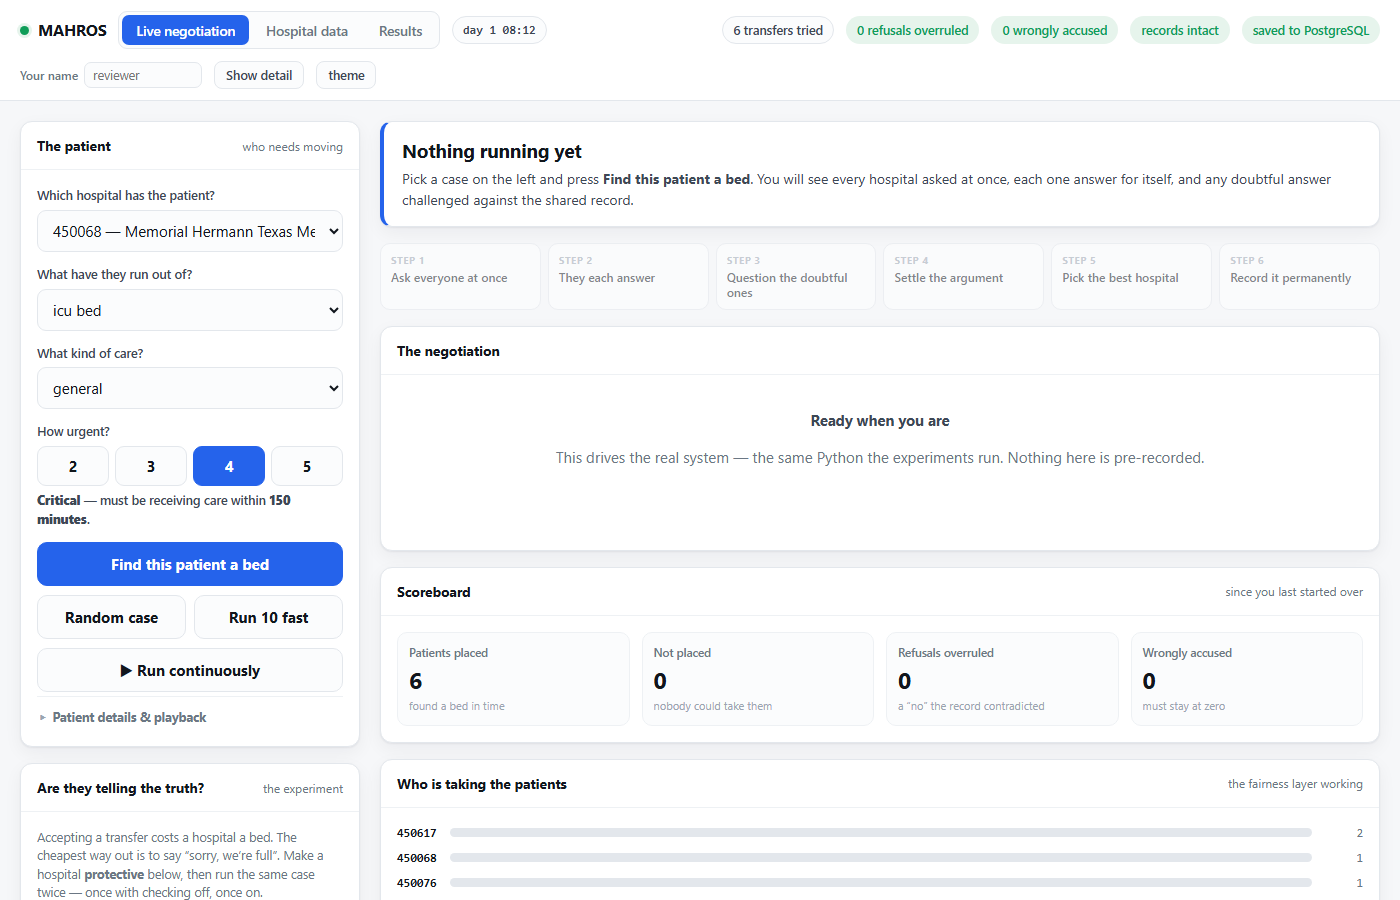
\includegraphics[width=0.78\textwidth]{figures/console.png}
\caption{The \mahros{} live console (Live negotiation tab) connected to PostgreSQL. Left: the case to place. Centre: the six protocol steps and a scoreboard of placements, overruled refusals and wrongly accused hospitals. Top right: record integrity and persistence status.}
\label{fig:console}
\end{figure*}
